\documentclass{article}

% packages
\usepackage{amsmath, amsthm, thmtools, amsfonts, amssymb, luacode, catchfile, tikzducks, hyperref, ifthen}
\ifcsname c@kobocompile\endcsname
	\usepackage[a5paper, total={1072pt, 1448pt}, margin=10pt, includeheadfoot]{geometry} % set page margins
\else
	\usepackage[a4paper, margin=50pt, includeheadfoot]{geometry}
\fi
\usepackage[shortlabels]{enumitem}
\usepackage[skip=3pt, indent=0pt]{parskip}

% language
\usepackage[bidi=basic, layout=tabular, provide=*]{babel}
\ifcsname c@english\endcsname
	\babelprovide[main, import]{english}
\else
	\babelprovide[main, import]{hebrew}
	\babelprovide{rl}
\fi
%\babelfont{rm}{Libertinus Serif}
\babelfont{rm}[Renderer=Harfbuzz]{Libertinus Serif}
\babelfont{sf}{Libertinus Sans}
\babelfont{tt}{Libertinus Mono}

% style
\AddToHook{cmd/section/before}{\clearpage}	% Add line break before section
\linespread{1.3}
\setcounter{secnumdepth}{0}		% Remove default number tags from sections, this won't do well with theorems
\AtBeginDocument{\setlength{\belowdisplayskip}{3pt}}
\AtBeginDocument{\setlength{\abovedisplayskip}{3pt}}
\graphicspath{ {../images/} }

% operators
\DeclareMathOperator\cis{cis}
\DeclareMathOperator\Sp{Sp}
\DeclareMathOperator\tr{tr}
\DeclareMathOperator\im{Im}
\DeclareMathOperator\re{Re}
\DeclareMathOperator\diag{diag}
\DeclareMathOperator*\lowlim{\underline{lim}}
\DeclareMathOperator*\uplim{\overline{lim}}
\DeclareMathOperator\rng{rng}
\DeclareMathOperator\Sym{Sym}
\DeclareMathOperator\Arg{Arg}
\DeclareMathOperator\Log{Log}
\DeclareMathOperator\dom{dom}
\DeclareMathOperator\supp{Supp}
\DeclareMathOperator\var{Var}
\DeclareMathOperator\cov{Cov}

% commands
%\renewcommand\qedsymbol{\textbf{מש''ל}}
%\renewcommand\qedsymbol{\fbox{\emoji{lizard}}}
\newcommand{\Aa}[0]{\mathcal{A}}
\newcommand{\Bb}[0]{\mathcal{B}}
\newcommand{\CC}[0]{\mathbb{C}}
\newcommand{\Cc}[0]{\mathcal{C}}
\newcommand{\EE}[0]{\mathbb{E}}
\newcommand{\FF}[0]{\mathbb{F}}
\newcommand{\Ff}[0]{\mathcal{F}}
\newcommand{\Ii}[0]{\mathcal{I}}
\newcommand{\Gg}[0]{\mathcal{G}}
\newcommand{\Ll}[0]{\mathcal{L}}
\newcommand{\Mm}[0]{\mathcal{M}}
\newcommand{\NN}[0]{\mathbb{N}}
\newcommand{\Nn}[0]{\mathcal{N}}
\newcommand{\PP}[0]{\mathbb{P}}
\newcommand{\Pp}[0]{\mathcal{P}}
\newcommand{\QQ}[0]{\mathbb{Q}}
\newcommand{\RR}[0]{\mathbb{R}}
\newcommand{\Rr}[0]{\mathcal{R}}
\newcommand{\Ss}[0]{\mathcal{S}}
\newcommand{\TT}[0]{\mathbb{T}}
\newcommand{\Uu}[0]{\mathcal{U}}
\newcommand{\Vv}[0]{\mathcal{V}}
\newcommand{\Ww}[0]{\mathcal{W}}
\newcommand{\ZZ}[0]{\mathbb{Z}}
\newcommand{\acts}[0]{\circlearrowright}
\newcommand{\explain}[2] {
	\begin{flalign*}
		 && \text{#2} && \text{#1}
	\end{flalign*}
}
\newcommand{\maketitleprint}[0]{ \begin{center}
	%\begin{tikzpicture}[scale=3]
	%	\duck[graduate=gray!20!black, tassel=red!70!black]
	%\end{tikzpicture}	
	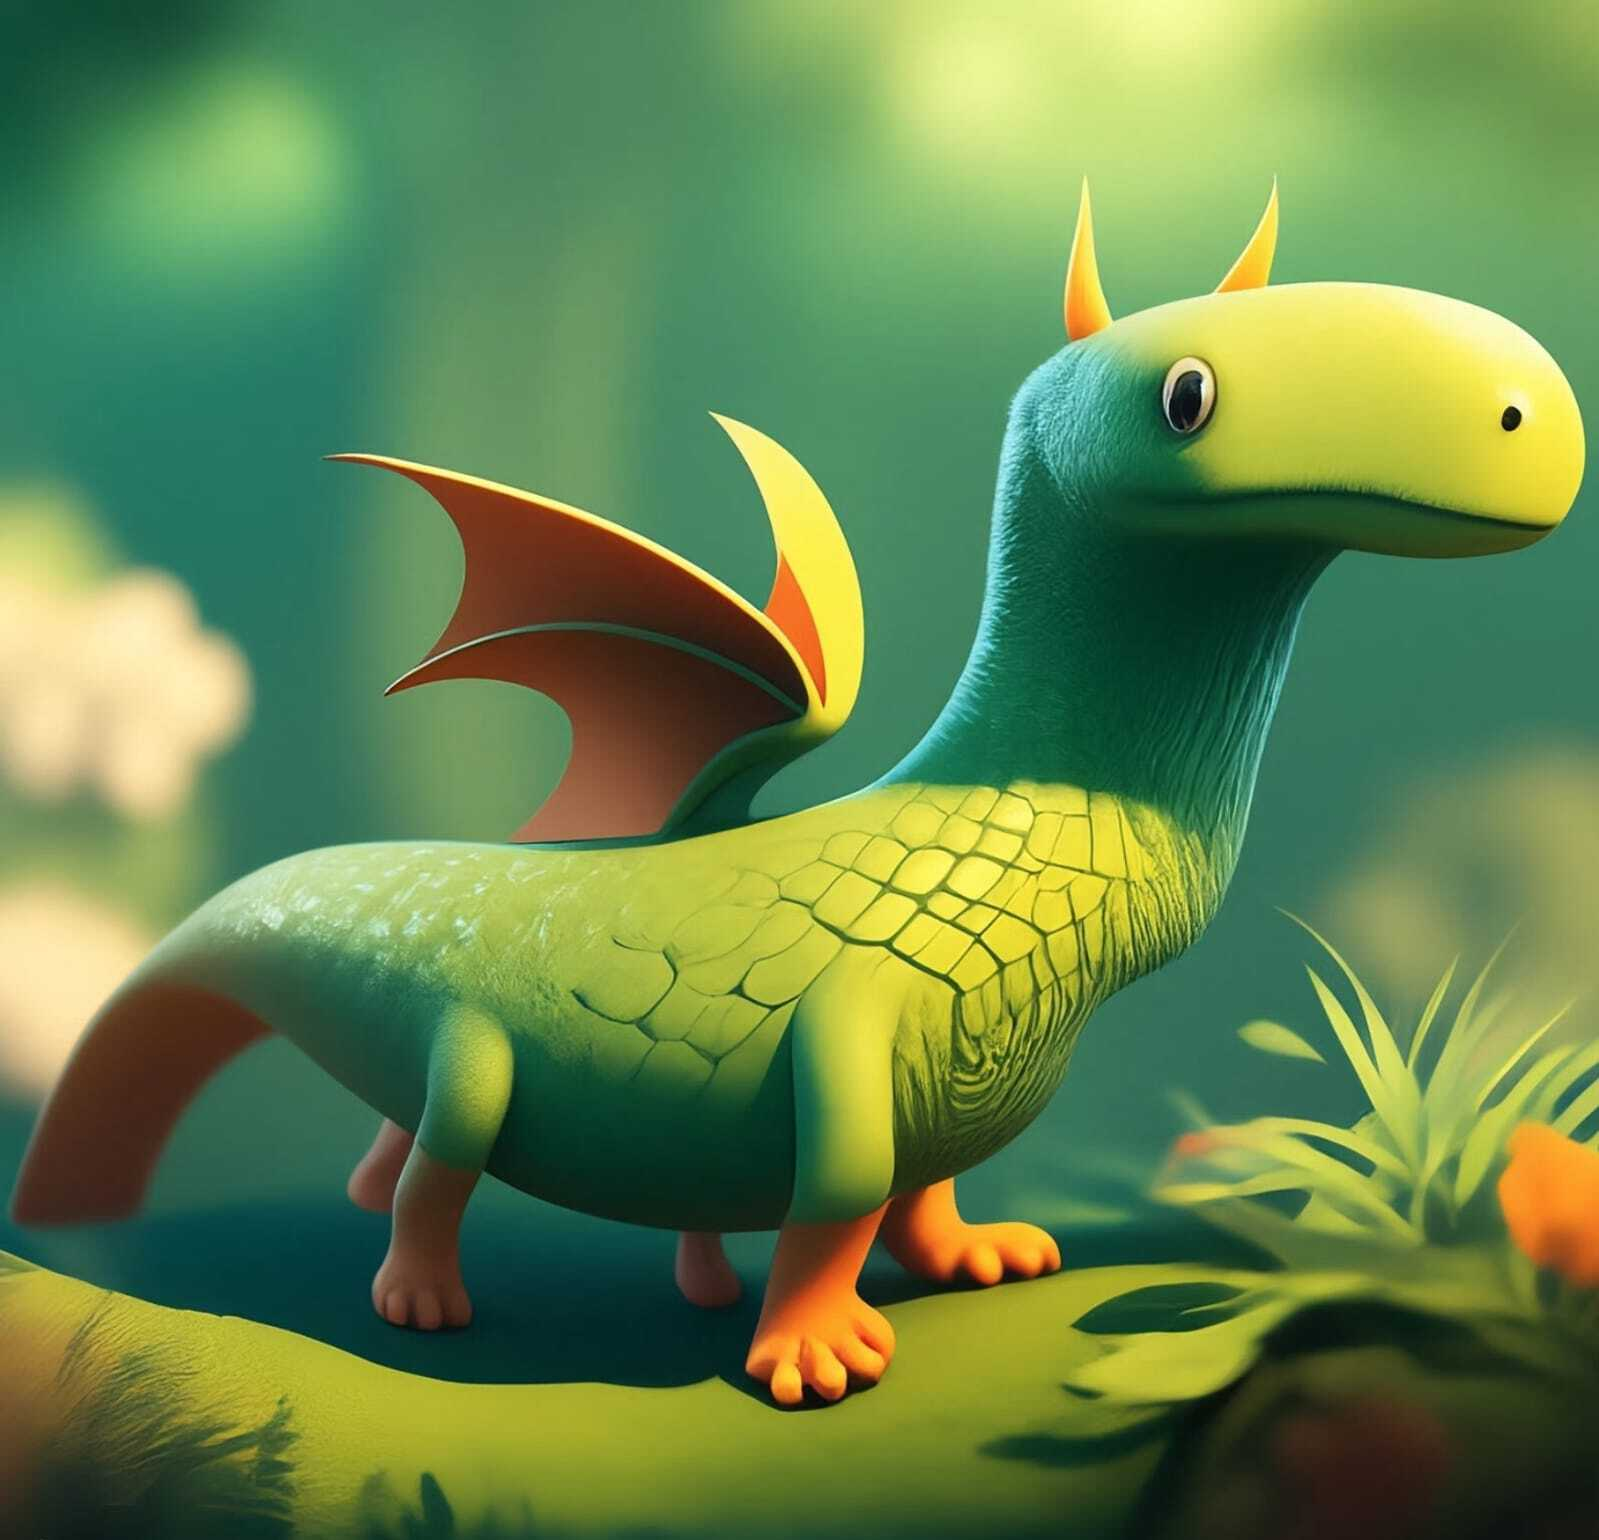
\includegraphics[width=6cm]{cover}
\end{center}
}

% theorem commands
\newtheoremstyle{c_remark}
	{}	% Space above
	{}	% Space below
	{}% Body font
	{}	% Indent amount
	{\bfseries}	% Theorem head font
	{}	% Punctuation after theorem head
	{.5em}	% Space after theorem head
	{\thmname{#1}\thmnumber{ #2}\thmnote{ \normalfont{\text{(#3)}}}}	% head content
\newtheoremstyle{c_definition}
	{3pt}	% Space above
	{3pt}	% Space below
	{}% Body font
	{}	% Indent amount
	{\bfseries}	% Theorem head font
	{}	% Punctuation after theorem head
	{.5em}	% Space after theorem head
	{\thmname{#1}\thmnumber{ #2}\thmnote{ \normalfont{\text{(#3)}}}}	% head content
\newtheoremstyle{c_plain}
	{3pt}	% Space above
	{3pt}	% Space below
	{\itshape}% Body font
	{}	% Indent amount
	{\bfseries}	% Theorem head font
	{}	% Punctuation after theorem head
	{.5em}	% Space after theorem head
	{\thmname{#1}\thmnumber{ #2}\thmnote{ \text{(#3)}}}	% head content

\ifcsname c@english\endcsname
	\theoremstyle{plain}
	\newtheorem{theorem}{Theorem}[section]
	\newtheorem{lemma}[theorem]{Lemma}
	\newtheorem{proposition}[theorem]{Proposition}
	\newtheorem*{proposition*}{Proposition}
	%\newtheorem{corollary}[theorem]{אין חלופה עברית}

	\theoremstyle{definition}
	\newtheorem{definition}[theorem]{Definition}
	\newtheorem*{definition*}{Definition}
	\newtheorem{example}{Example}[section]
	\newtheorem{exercise}{Exercise}[section]

	\theoremstyle{remark}
	\newtheorem*{remark}{Remark}
	\newtheorem*{solution}{Solution}
	\newtheorem{conclusion}[theorem]{Conclusion}
	\newtheorem{notation}[theorem]{Notation}
\else
	\theoremstyle{c_plain}
	\newtheorem{theorem}{משפט}[section]
	\newtheorem{lemma}[theorem]{למה}
	\newtheorem{proposition}[theorem]{טענה}
	\newtheorem*{proposition*}{טענה}
	%\newtheorem{corollary}[theorem]{אין חלופה עברית}

	\theoremstyle{c_definition}
	\newtheorem{definition}[theorem]{הגדרה}
	\newtheorem*{definition*}{הגדרה}
	\newtheorem{example}{דוגמה}[section]
	\newtheorem{exercise}{תרגיל}[section]

	\theoremstyle{c_remark}
	\newtheorem*{remark}{הערה}
	\newtheorem*{solution}{פתרון}
	\newtheorem{conclusion}[theorem]{מסקנה}
	\newtheorem{notation}[theorem]{סימון}
\fi

% Questions related commands
\newcounter{question}
\setcounter{question}{1}
\newcounter{sub_question}
\setcounter{sub_question}{1}

\ifcsname c@english\endcsname
	\newcommand{\question}[1][0]{
		\ifthenelse{#1 = 0}{}{\setcounter{question}{#1}}
		\section{Question \arabic{question}}
		\addtocounter{question}{1}
		\setcounter{sub_question}{1}
	}

	\newcommand{\subquestion}[1][0]{
		\ifthenelse{#1 = 0}{}{\setcounter{sub_question}{#1}}
		\subsection{Part \alph{sub_question}}
		\addtocounter{sub_question}{1}
	}
\else
	\newcommand{\question}[1][0]{
		\ifthenelse{#1 = 0}{}{\setcounter{question}{#1}}
		\section{שאלה \arabic{question}}
		\addtocounter{question}{1}
		\setcounter{sub_question}{1}
	}

	\newcommand{\subquestion}[1][0]{
		\ifthenelse{#1 = 0}{}{\setcounter{sub_question}{#1}}
		\subsection{סעיף \localecounter{letters.gershayim}{sub_question}}
		\addtocounter{sub_question}{1}
	}
\fi

% import lua and start of document
\directlua{common = require ('../common')}

\GetEnv{AUTHOR}

% headers
\author{\AUTHOR}
\date\today

\title{פתרון מטלה 08 --- מבוא ללוגיקה, 80423}

\begin{document}
\maketitle
\maketitleprint{}

\question{}
תהי $L$ שפה לתחשיב יחסים, תהי $\varphi$ נוסחה ונניח ש־$x \in Var$.

\subquestion{}
נוכיח שלכל מבנה $\mathcal{A}$ ל־$L$ ולכל השמה $\sigma : Var \to A$ מתקיים $\mathcal{A} \models \varphi(\sigma)$, אם ורק אם לכל מבנה והשמה כאלה מתקיים $\mathcal{A} \models \forall x \varphi(\sigma)$.
\begin{proof}
	נניח את הכיוון הראשון, נקבע $\mathcal{A}$ כלשהו ונבחין כי $\mathcal{A} \models \varphi(\sigma)$ לכל הצבה $\sigma$ כזו.
	לכן בפרט לכ הצבה, גם $\mathcal{A} \models \varphi(\sigma[x : a])$ לכל $a \in A$.
	אבל במצב זה נבחין כי לכל $a \in A$ הטענה מתקיימת, כלומר $\mathcal{A} \models \forall x \varphi(\sigma)$, ומצאנו כי הטענה אכן חלה.

	לכיוון ההפוך נקבע שוב $\mathcal{A}$ כזה המקיים את הטענה והפעם נקבל שאם $\mathcal{A} \models \forall x \varphi(\sigma)$ אז בפרט לכל $a \in A$ מתקיים $\mathcal{A} \models \varphi(\sigma[x : a])$.
	נוכל אם כן לבנות כל $\sigma : Var \to A$ כך ש־$\mathcal{A} \models \varphi(\sigma)$.
\end{proof}

\subquestion{}
נוכיח שלכל מבנה $\mathcal{A}$ ל־$L$ ולכל השמה $\sigma : Var \to A$ מתקיים $\mathcal{A} \models \varphi(\sigma)$ אם ורק אם לכל הכללה $\psi$ של $\varphi$ ולכל מבנה $\mathcal{A}$ ל־$L$ מתקיים $\mathcal{A} \models \psi$.
\begin{proof}
	נוכיח את הטענה באינדוקציה. \\
	נבחין כי בסיס האינדוקציה הוא למעשה טענת הסעיף הקודם, ולכן נסיק שהיא אכן חלה. \\
	נניח ש־$FV(\varphi) = \{ x_0, \dots, x_{n - 1} \}$ וכן ש־$\psi = \forall x_0 \dots \forall x_{n - 2} \varphi(x_0, \dots, x_{n - 1})$ ושהטענה חלה עבור פסוקים אלה, ונבחן את $\phi = \forall x_{n - 1} \psi(x_{n - 1})$.
	אז מאותה הוכחה של סעיף א' נובע שהטענה מתקיימת עבור $\phi$ ביחס ל־$\psi$ ולכן השלמנו את מהלך האינדוקציה.
\end{proof}

\question{}
תהי $L = \{ p_0, \dots, p_{n - 1} \}$ שפה לתחשיב פסוקים, $\alpha \in form_L$. \\
תהי $L'$ שפה לתחשיב יחסים ו־$\varphi_0, \dots, \varphi_{n - 1} \in form_{L'}$. \\
תהי $\alpha_{\varphi_0, \dots, \varphi_{n - 1}}^{p_0, \dots, p_{n - 1}}$ נוסחה המתקבלת מהחלפת כל מופע של $p_i$ ב־$\varphi_i$ בו־זמנית.

\subquestion{}
נוכיח שזוהי אכן נוסחה.
\begin{proof}
	נוכיח באינדוקציה על מבנה הפסוק בתחשיב פסוקים. \\
	עבור הבסיס נניח ש־$\alpha = p_i$ עבור $i \in [n]$, ולכן מההגדרה $\alpha_{\varphi_0, \dots, \varphi_{n - 1}}^{p_0, \dots, p_{n - 1}} = \varphi_i$ וזוהי כמובן נוסחה. \\
	נניח שהטענה מתקיימת עבור $\alpha$ ונבחן את $(\lnot \alpha)$. נניח $\alpha_{\varphi_0, \dots, \varphi_{n - 1}}^{p_0, \dots, p_{n - 1}} = \psi$,
	ולכן מההגדרה ${(\lnot \alpha)}_{\varphi_0, \dots, \varphi_{n - 1}}^{p_0, \dots, p_{n - 1}} = (\lnot \psi)$ וזוהי כמובן נוסחה. \\
	באופן דומה אם $\alpha, \beta$ מקיימות את הטענה אז קיימות החלפות $\psi_0, \psi_1$ בהתאמה עבורן, וברור ש־$(\psi_0 \square \psi_1)$ נוסחה לכל $\square \in \mathcal{B}$,
	אבל זוהי גם תוצאת ההחלפה של $(\alpha \square \beta)$, ולכן השלמנו את מהלך האינדוקציה והטענה אכן מתקיימת.
\end{proof}

\subquestion{}
נוכיח שאם $\alpha$ טאוטולוגיה אז גם $\alpha_{\varphi_0, \dots, \varphi_{n - 1}}^{p_0, \dots, p_{n - 1}}$ היא טאוטולוגיה כנוסחה ב־$L$.
\begin{proof}
	נבחין כי יש משמעות לשאילת שאלה זו בשל תוצאת הסעיף הקודם.
	נניח ש־$f : form_L \to form_{L'}$ ההחלפה שהגדרנו קודם לכן, ונגדיר גם $g : form_{L'} \to form_{L_{prop}'}$ הבנייה שהגדרנו בהרצאה להחלפת נוסחות יסודיות.
	נבחין ש־$g \circ f$ היא פונקציה $form_L \to form_{L_{prop}'}$ פונקציית החלפה בין שפות בתחשיב פסוקים המקיימות את טענת שאלה 1 במטלה 3, לכן הרכבה זו משמרת שקילות טאוטולוגית.
	כלומר אם $\alpha$ טאוטולוגיה אז גם $(g \circ f)(\alpha)$ כפי שרצינו להראות.
\end{proof}

\subquestion{}
נסיק שנוסחה בשפה לתחשיב יחסים היא טאוטולוגיה אם ורק אם היא מהצורה $\alpha_{\varphi_0, \dots, \varphi_{n - 1}}^{p_0, \dots, p_{n - 1}}$ עבור טאוטולוגיה $\alpha$ ושפה כלשהי לתחשיב פסוקים $L'$.
\begin{proof}
	נניח את הכיוון הראשון ולכן משאלה 1 במטלה 3 נוכל להחליף את פסוקיה היסודיים בכל נוסחה תקינה על־פי המוגדר ונקבל נוסחה שהיא טאוטולוגיה מעל תחשיב פסוקים.

	נקבל נוסחה שהיא תוצאת החלפה עבור של טאוטולוגיה נסיק מהסעיף הקודם את המבוקש.
\end{proof}

\question{}
תהי שפה $L$ לתחשיב פסוקים ויהיו $\psi_0, \psi_1 \in form_L$, נוכיח שאם $\vdash \psi_0$ וגם $\vdash (\psi_0 \to \psi_1)$ אז $\vdash \psi_1$.
\begin{proof}
	נתון כי קיים עץ היסק עבור $\psi_0, (\psi_0 \to \psi_1)$, עץ זה הוא סופי ואנו יכולים לשרשר אותו לתוך עצים אחרים, אז נבנה את עץ ההיסק
	\begin{enumerate}
		\item $\lnot \psi_1$
		\item פיצול למקרים על $\psi_0$
			\begin{enumerate}
				\item $\psi_0$
				\item פיצול למקרים על $(\psi_0 \to \psi_1)$
					\begin{enumerate}
						\item $(\psi_0 \to \psi_1)$
						\item $\psi_1$, כלל היסק לגרירה (מודוס פוננס) וסתירה
					\end{enumerate}
					\begin{enumerate}
						\item $\lnot (\psi_0 \to \psi_1)$
						\item חזרה על כלל העץ עבור $(\psi_0 \to \psi_1)$, למעשה כל מה שמופיע החל מפה יופיע כהמשכים של כלל העלים בעץ הזה, מטעמי נוחות לא נכתוב זאת כך
						\item $(\psi_0 \to \psi_1)$ וסתירה
					\end{enumerate}
			\end{enumerate}
			\begin{enumerate}
				\item $\lnot \psi_0$
				\item חזרה על כלל העץ עבור $\psi_0$, למעשה כל מה שמופיע החל מפה יופיע כהמשכים של כלל העלים בעץ הזה, מטעמי נוחות לא נכתוב זאת כך
				\item $\psi_0$ וסתירה
			\end{enumerate}
	\end{enumerate}
	הגענו לסתירה בכל ענף ולכן עץ היסק זה מעיד על $\vdash \psi_1$.
\end{proof}

\question{}
תהי $L$ שפה לתחשיב פסוקים ויהיו $\psi_0, \psi_1, \psi_2 \in form_L$, בסעיפים הבאים נכתוב עצי היסק במערכת ההיסק KEP עבור כל טענה.

\subquestion{}
$\psi_0 \vdash (\psi_0 \lor \psi_1)$.
\begin{solution}
	נבנה את עץ ההיסק המתאים.
	\begin{enumerate}
		\item $\lnot (\psi_0 \lor \psi_1)$
		\item $\lnot \psi_0$, כללי איווי
		\item $\psi_0$, הוספת הנחה, וסתירה
	\end{enumerate}
\end{solution}

\subquestion{}
$(\psi_0 \lor \psi_1) \vdash (\psi_1 \lor \psi_0)$.
\begin{solution}
	נבנה את עץ ההיסק המתאים.
	\begin{enumerate}
		\item $\lnot (\psi_1 \lor \psi_0)$
		\item $\lnot \psi_0$, כללי איווי
		\item $(\psi_0 \lor \psi_1)$, הוספת הנחה
		\item $\psi_0$, כללי איווי וסתירה
	\end{enumerate}
	נבחין כי יכולנו גם לפצל למקרים על ערך $\psi_0$ ו־$\psi_1$ כדי לבנות עץ היסק שמתיישב יותר טוב עם הדרך שבה אנו מוכיחים.
\end{solution}

\subquestion{}
$((\psi_0 \lor \psi_1) \lor \psi_2) \vdash (\psi_0 \lor (\psi_1 \lor \psi_2))$.
\begin{solution}
	נבנה את עץ ההיסק המתאים.
	\begin{enumerate}
		\item $\lnot (\psi_0 \lor (\psi_1 \lor \psi_2))$
		\item $\lnot (\psi_1 \lor \psi_2)$, כללי איווי
		\item $\lnot \psi_2$, כללי איווי
		\item $((\psi_0 \lor \psi_1) \lor \psi_2)$, הוספת הנחה
		\item $\psi_2$, כללי איווי, וסתירה
	\end{enumerate}
\end{solution}

\subquestion{}
$((\psi_0 \land \psi_1) \land \psi_2) \vdash (\psi_0 \land (\psi_1 \land \psi_2))$.
\begin{solution}
	נבנה את עץ ההיסק המתאים.
	\begin{enumerate}
		\item $\lnot (\psi_0 \land (\psi_1 \land \psi_2))$
		\item $(\psi_0 \land \psi_1) \land \psi_2$, הוספת הנחה
		\item $\psi_2$, כללי גימום
		\item פיצול למקרים $\psi_0$
			\begin{enumerate}
				\item $\psi_0$
				\item $\lnot (\psi_1 \land \psi_2)$, כללי גימום
				\item פיצול למקרים $\psi_1$
					\begin{enumerate}
						\item $\psi_1$
						\item $\lnot \psi_2$, כללי גימום וסתירה
					\end{enumerate}
					\begin{enumerate}
						\item $\lnot \psi_1$
						\item $(\psi_0 \land \psi_1)$ כללי גימום מ־2
						\item $\psi_1$, כללי גימום, וסתירה
					\end{enumerate}
			\end{enumerate}
			\begin{enumerate}
				\item $\lnot \psi_0$
				\item $\psi_0 \land \psi_1$, כללי גימום מ־2
				\item $\psi_0$, כללי גימום, סתירה
			\end{enumerate}
	\end{enumerate}
\end{solution}

\subquestion{}
$\vdash (((\psi_0 \lor \psi_1) \land \psi_2) \leftrightarrow ((\psi_0 \land \psi_2) \lor (\psi_1 \land \psi_2)))$.
\begin{solution}
	נבנה את עץ ההיסק המתאים.
	\begin{enumerate}
		\item $\lnot (((\psi_0 \lor \psi_1) \land \psi_2) \leftrightarrow ((\psi_0 \land \psi_2) \lor (\psi_1 \land \psi_2)))$.
		\item פיצול למקרים $((\psi_0 \lor \psi_1) \land \psi_2)$
			\begin{enumerate}
				\item $((\psi_0 \lor \psi_1) \land \psi_2)$
				\item $\psi_2$
				\item $\lnot ((\psi_0 \land \psi_2) \lor (\psi_1 \land \psi_2))$, כללי גרירה דו־כיוונית
				\item $\lnot (\psi_0 \land \psi_2)$
				\item פיצול למקרים על $\psi_0$
					\begin{enumerate}
						\item $\psi_0$
						\item $\lnot \psi_2$, כללי גימום, וסתירה
					\end{enumerate}
					\begin{enumerate}
						\item $\lnot \psi_0$
						\item $\psi_0 \lor \psi_1$, כללי גימום מ־a
						\item $\psi_1$, כללי איווי
						\item $\lnot (\psi_1 \land \psi_2)$, כללי איווי
						\item $\lnot \psi_2$, כללי גימום, סתירה
					\end{enumerate}
			\end{enumerate}
			\begin{enumerate}
				\item $\lnot ((\psi_0 \lor \psi_1) \land \psi_2)$
				\item $\lnot (\psi_0 \lor \psi_1)$, כללי גימום
				\item $\lnot \psi_0$, כללי איווי
				\item $(\psi_0 \land \psi_2) \lor (\psi_1 \land \psi_2)$, כללי גרירה דו־כיוונית
				\item פיצול למקרים על $(\psi_0 \land \psi_2)$
					\begin{enumerate}
						\item $\psi_0 \land \psi_2$
						\item $\psi_0$, כללי גימום, סתירה
					\end{enumerate}
					\begin{enumerate}
						\item $\lnot (\psi_0 \land \psi_2)$
						\item $\psi_1 \land \psi_2$, כללי איווי
						\item $\psi_1$, כללי גימום
						\item $\lnot \psi_1$, כללי איווי ל־b, וסתירה
					\end{enumerate}
			\end{enumerate}
	\end{enumerate}
\end{solution}

\subquestion{}
$(\psi_0 \to \psi_1), (\psi_1 \to \psi_0) \vdash (\psi_0 \leftrightarrow \psi_1)$.
\begin{solution}
	נבנה את עץ ההיסק המתאים.
	\begin{enumerate}
		\item $\lnot (\psi_0 \leftrightarrow \psi_1)$
		\item פיצול למקרים על $\psi_0$
			\begin{enumerate}
				\item $\psi_0$
				\item $\lnot \psi_1$, כללי גרירה דו־כיוונית
				\item $\psi_0 \to \psi_1$, הוספת הנחה
				\item $\psi_1$, כללי גרירה, סתירה
			\end{enumerate}
			\begin{enumerate}
				\item $\lnot \psi_0$
				\item $\psi_1$, כללי גרירה דו־כיוונית
				\item $\psi_1 \to \psi_0$, הוספת הנחה
				\item $\lnot \psi_1$, חוקי גרירה, סתירה
			\end{enumerate}
	\end{enumerate}
\end{solution}

\subquestion{}
$\vdash ((\psi_0 \land (\lnot \psi_0)) \to (\psi_1 \land (\lnot \psi_1)))$.
\begin{solution}
	נבנה את עץ ההיסק המתאים.
	\begin{enumerate}
		\item $\lnot ((\psi_0 \land (\lnot \psi_0)) \to (\psi_1 \land (\lnot \psi_1)))$
		\item $\psi_0 \land (\lnot \psi_0)$, חוקי גרירה
		\item $\psi_0$, חוקי גימום
		\item $\lnot \psi_0$, חוקי גימום, סתירה
	\end{enumerate}
\end{solution}

\subquestion{}
$\vdash (\psi_0 \to (\psi_1 \to \psi_0))$.
\begin{solution}
	נבנה את עץ ההיסק המתאים.
	\begin{enumerate}
		\item $\lnot (\psi_0 \to (\psi_1 \to \psi_0))$
		\item $\psi_0$, כללי גרירה
		\item $\lnot (\psi_1 \to \psi_0)$, כללי גרירה ל־1
		\item $\lnot \psi_0$, כללי גרירה, וסתירה
	\end{enumerate}
\end{solution}

\subquestion{}
$\vdash (((\lnot \psi_0) \to (\lnot \psi_1)) \to (\psi_1 \to \psi_0))$.
\begin{solution}
	נבנה את עץ ההיסק המתאים.
	\begin{enumerate}
		\item $\lnot (((\lnot \psi_0) \to (\lnot \psi_1)) \to (\psi_1 \to \psi_0))$
		\item $(\lnot \psi_0) \to (\lnot \psi_1)$, כללי גרירה
		\item $\lnot (\psi_1 \to \psi_0)$, כללי גרירה ל־1
		\item $\psi_1$, כללי גרירה
		\item $\lnot \psi_0$, כללי גרירה
		\item $\lnot \psi_1$, כללי גרירה ל־2, וסתירה
	\end{enumerate}
\end{solution}

\subquestion{}
$\vdash ((\psi_0 \to (\psi_1 \to \psi_2)) \to ((\psi_0 \to \psi_1) \to (\psi_0 \to \psi_2)))$.
\begin{solution}
	נבנה את עץ ההיסק המתאים.
	\begin{enumerate}
		\item $\lnot ((\psi_0 \to (\psi_1 \to \psi_2)) \to ((\psi_0 \to \psi_1) \to (\psi_0 \to \psi_2)))$
		\item $\psi_0 \to (\psi_1 \to \psi_2)$, חוקי גרירה
		\item $\lnot ((\psi_0 \to \psi_1) \to (\psi_0 \to \psi_2))$, חוקי גרירה ל־1
		\item $\psi_0 \to \psi_1$, חוקי גרירה
		\item $\lnot (\psi_0 \to \psi_2)$, חוקי גרירה
		\item $\psi_0$, חוקי גרירה
		\item $\lnot \psi_2$, חוקי גרירה
		\item $\psi_1$, חוקי גרירה ל־4
		\item $\psi_1 \to \psi_2$, חוקי גרירה ל־2
		\item $\psi_2$, חוקי גרירה, וסתירה
	\end{enumerate}
\end{solution}

\question{}
נאמר שכלל היסק ניתן להשמטה אם כל שפה $L$ לתחשיב פסוקים ולכל קבוצת פסוקים $\Sigma$ ופסוק $\varphi$ כך ש־$\Sigma \vdash \varphi$ קיים עץ היסק לטענה כך שהכלל אינו מופיע בה, לכל כלל בסעיפים הבאים נוכיח שהוא ניתן להשמטה.

\subquestion{}
$\frac{(A \to B), (\lnot B)}{(\lnot A)}$
\begin{proof}
	כדי להראות שכלל היסק ניתן להשמטה די שנראה שבכל עץ בו הוא מופיע, ניתן לבנות עץ חדש ללא הכלל, כך שתוצאתו תמשיך להיות תקפה.
	לשם כך אנו נניח שישנו עץ היסק בו יש שימוש בטענה זו, ועתה נבנה עץ שיחליף את העץ הזה ושמשתמש בכללי ההיסק הנתונים לנו כרגע
	\begin{enumerate}
		\item $A \to B$, כלל החזרה
		\item חלוקה למקרים על $A$
			\begin{enumerate}
				\item $A$
				\item $B$, כללי גרירה ל־1
				\item $\lnot B$, כלל החזרה, וסתירה
			\end{enumerate}
			\begin{enumerate}
				\item $\lnot A$
				\item נקודת ההחלפה השנייה
			\end{enumerate}
	\end{enumerate}
	מצאנו עץ היסק שניתן להחליף את כלל ההיסק הרצוי בו, כך שהטענות נשארות ללא שינוי, נבחין שוב כי זוהי פעולת החלפה עבור עצים בינאריים, וכי היא תקפה, בסעיפים הבאים נשתמש באותה הטענה בדיוק, אך ללא הסבר זה
	נקודת ההחלפה השנייה היא כלל חלקי העץ שמגעים אחרי ההיסק שהחלפנו, צלע זו תוחלף בו, וכך יתקבל עץ היסק מלא כך שאכן יש סתירה בעל ענף.
\end{proof}

\subquestion{}
$\frac{(A \leftrightarrow B), A}{B}$
\begin{proof}
	נבנה את חלק עץ ההיסק להחלפה
	\begin{enumerate}
		\item $A \leftrightarrow B$, כלל החזרה
		\item $A$, כלל החזרה
		\item פיצול למקרים על $B$
			\begin{enumerate}
				\item $B$
				\item נקודת ההחלפה השנייה
			\end{enumerate}
			\begin{enumerate}
				\item $\lnot B$
				\item $\lnot A$, כללי הגרירה הדו־כיוונית ל־1, וסתירה
			\end{enumerate}
	\end{enumerate}
\end{proof}

\subquestion{}
$\frac{(A \leftrightarrow B), (\lnot B)}{(\lnot A)}$
\begin{proof}
	גם הפעם נבנה את עץ ההיסק המחליף
	\begin{enumerate}
		\item $A \leftrightarrow B$, כלל החזרה
		\item $\lnot B$, כלל החזרה
		\item פיצול למקרים על $A$
			\begin{enumerate}
				\item $A$
				\item $B$, כללי גרירה דו־כיוונית ל־1, וסתירה
			\end{enumerate}
			\begin{enumerate}
				\item $\lnot A$
				\item נקודת ההחלפה השנייה
			\end{enumerate}
	\end{enumerate}
\end{proof}

\end{document}
